% Options for packages loaded elsewhere
\PassOptionsToPackage{unicode}{hyperref}
\PassOptionsToPackage{hyphens}{url}
%
\documentclass[
]{article}
\usepackage{amsmath,amssymb}
\usepackage{lmodern}
\usepackage{ifxetex,ifluatex}
\ifnum 0\ifxetex 1\fi\ifluatex 1\fi=0 % if pdftex
  \usepackage[T1]{fontenc}
  \usepackage[utf8]{inputenc}
  \usepackage{textcomp} % provide euro and other symbols
\else % if luatex or xetex
  \usepackage{unicode-math}
  \defaultfontfeatures{Scale=MatchLowercase}
  \defaultfontfeatures[\rmfamily]{Ligatures=TeX,Scale=1}
\fi
% Use upquote if available, for straight quotes in verbatim environments
\IfFileExists{upquote.sty}{\usepackage{upquote}}{}
\IfFileExists{microtype.sty}{% use microtype if available
  \usepackage[]{microtype}
  \UseMicrotypeSet[protrusion]{basicmath} % disable protrusion for tt fonts
}{}
\makeatletter
\@ifundefined{KOMAClassName}{% if non-KOMA class
  \IfFileExists{parskip.sty}{%
    \usepackage{parskip}
  }{% else
    \setlength{\parindent}{0pt}
    \setlength{\parskip}{6pt plus 2pt minus 1pt}}
}{% if KOMA class
  \KOMAoptions{parskip=half}}
\makeatother
\usepackage{xcolor}
\IfFileExists{xurl.sty}{\usepackage{xurl}}{} % add URL line breaks if available
\IfFileExists{bookmark.sty}{\usepackage{bookmark}}{\usepackage{hyperref}}
\hypersetup{
  pdftitle={Distribution of z-statistics},
  hidelinks,
  pdfcreator={LaTeX via pandoc}}
\urlstyle{same} % disable monospaced font for URLs
\usepackage[margin=1in]{geometry}
\usepackage{graphicx}
\makeatletter
\def\maxwidth{\ifdim\Gin@nat@width>\linewidth\linewidth\else\Gin@nat@width\fi}
\def\maxheight{\ifdim\Gin@nat@height>\textheight\textheight\else\Gin@nat@height\fi}
\makeatother
% Scale images if necessary, so that they will not overflow the page
% margins by default, and it is still possible to overwrite the defaults
% using explicit options in \includegraphics[width, height, ...]{}
\setkeys{Gin}{width=\maxwidth,height=\maxheight,keepaspectratio}
% Set default figure placement to htbp
\makeatletter
\def\fps@figure{htbp}
\makeatother
\setlength{\emergencystretch}{3em} % prevent overfull lines
\providecommand{\tightlist}{%
  \setlength{\itemsep}{0pt}\setlength{\parskip}{0pt}}
\setcounter{secnumdepth}{-\maxdimen} % remove section numbering
\ifluatex
  \usepackage{selnolig}  % disable illegal ligatures
\fi

\title{Distribution of z-statistics}
\author{}
\date{\vspace{-2.5em}}

\begin{document}
\maketitle

\hypertarget{all-4-methods-with-omited}{%
\section{All 4 methods with omited}\label{all-4-methods-with-omited}}

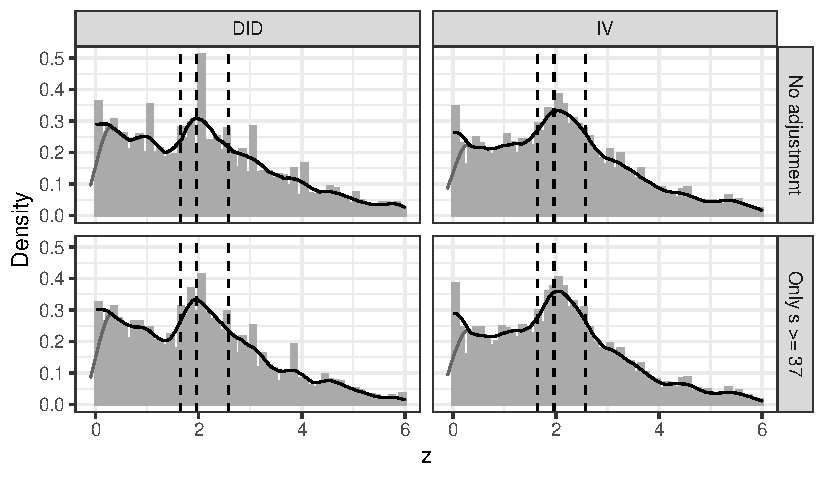
\includegraphics{C:/Users/ppuetz/Desktop/sciebo/methods_matter_replication/Submission AER/revision/comment_methods_matter/replication_repo_methods_matter_comment/Results/zplot_iv_did-1.pdf}

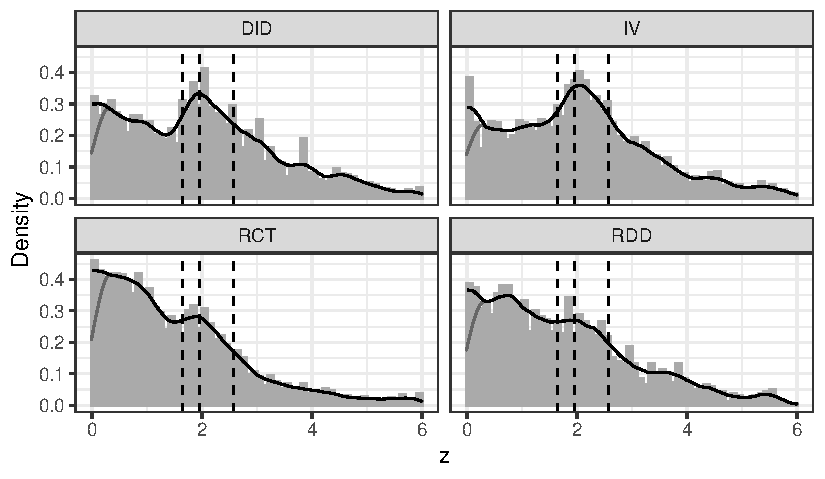
\includegraphics{C:/Users/ppuetz/Desktop/sciebo/methods_matter_replication/Submission AER/revision/comment_methods_matter/replication_repo_methods_matter_comment/Results/zplot_omit-1.pdf}

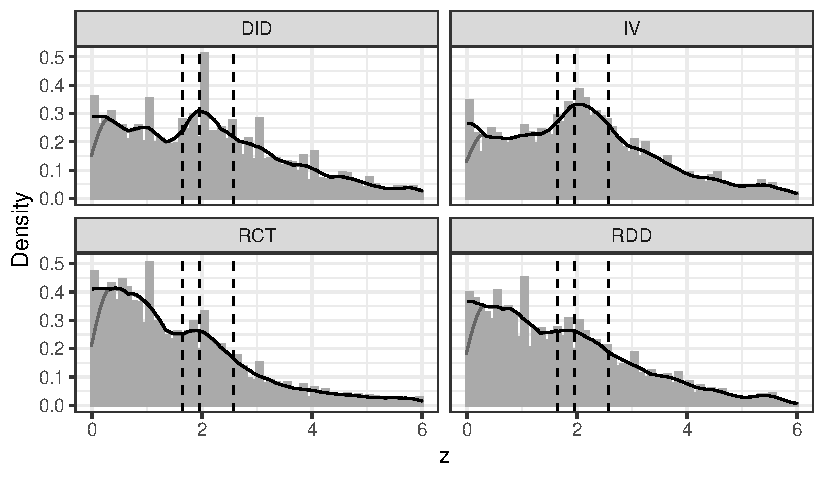
\includegraphics{C:/Users/ppuetz/Desktop/sciebo/methods_matter_replication/Submission AER/revision/comment_methods_matter/replication_repo_methods_matter_comment/Results/zplot_reported-1.pdf}

\hypertarget{distribution-of-z-tests-all-vs-non-omitted}{%
\section{Distribution of z-tests: All vs
non-omitted}\label{distribution-of-z-tests-all-vs-non-omitted}}

We see how the derounding approaches mainly remove the large clusters at
z=2.

\hypertarget{pooled}{%
\subsubsection{Pooled}\label{pooled}}

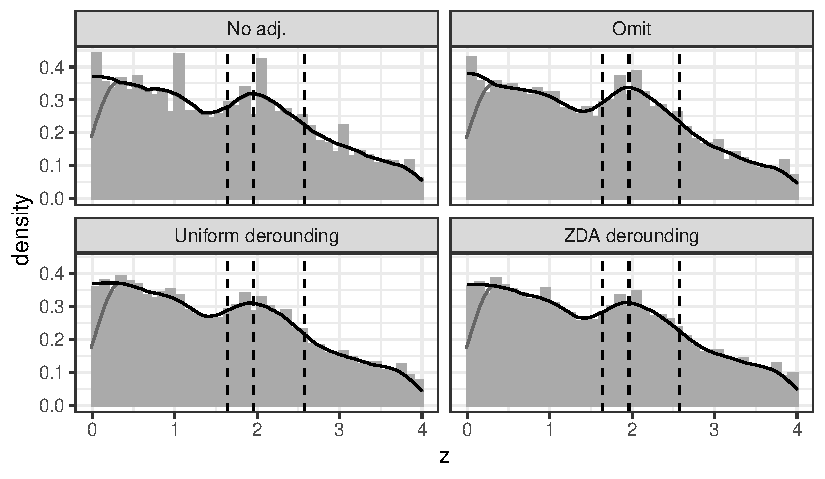
\includegraphics{C:/Users/ppuetz/Desktop/sciebo/methods_matter_replication/Submission AER/revision/comment_methods_matter/replication_repo_methods_matter_comment/Results/zplot_all-1.pdf}

\hypertarget{did}{%
\subsubsection{DID}\label{did}}

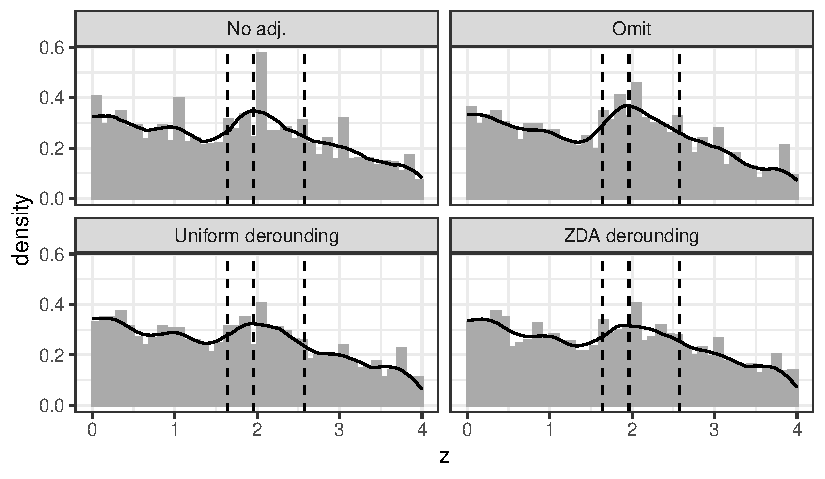
\includegraphics{C:/Users/ppuetz/Desktop/sciebo/methods_matter_replication/Submission AER/revision/comment_methods_matter/replication_repo_methods_matter_comment/Results/zplot_did-1.pdf}

\hypertarget{iv}{%
\subsubsection{IV}\label{iv}}

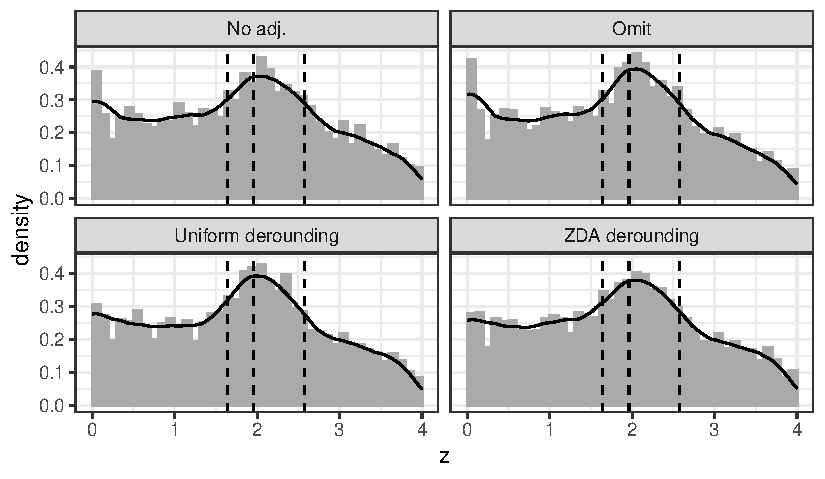
\includegraphics{C:/Users/ppuetz/Desktop/sciebo/methods_matter_replication/Submission AER/revision/comment_methods_matter/replication_repo_methods_matter_comment/Results/zplot_iv-1.pdf}

\hypertarget{rdd}{%
\subsubsection{RDD}\label{rdd}}

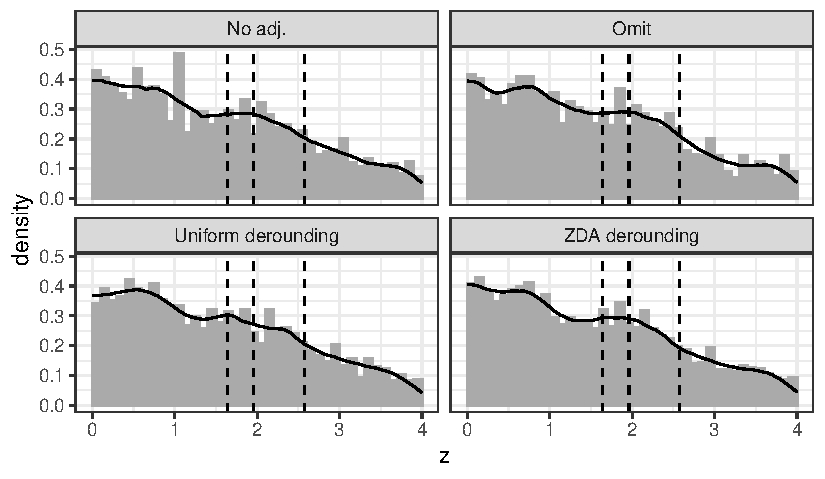
\includegraphics{C:/Users/ppuetz/Desktop/sciebo/methods_matter_replication/Submission AER/revision/comment_methods_matter/replication_repo_methods_matter_comment/Results/zplot_rdd-1.pdf}

\hypertarget{rct}{%
\subsubsection{RCT}\label{rct}}

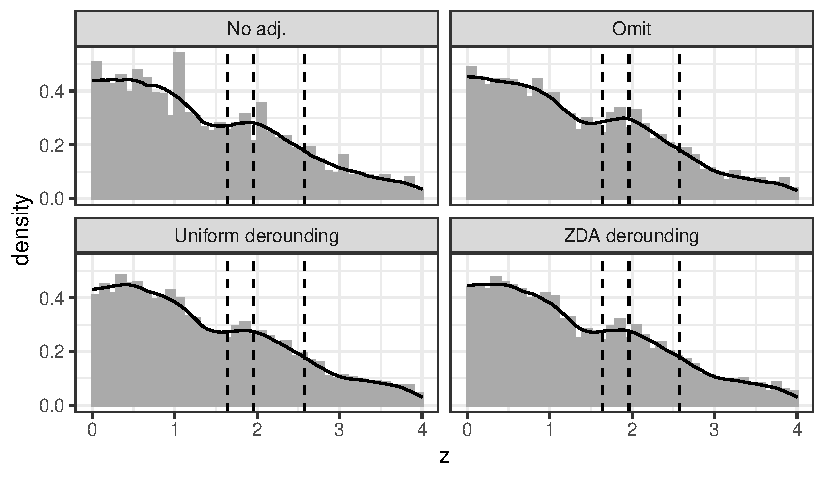
\includegraphics{C:/Users/ppuetz/Desktop/sciebo/methods_matter_replication/Submission AER/revision/comment_methods_matter/replication_repo_methods_matter_comment/Results/zplot_rct-1.pdf}

\hypertarget{same-plots-with-larger-z-range}{%
\section{Same plots with larger z
range}\label{same-plots-with-larger-z-range}}

\hypertarget{pooled-1}{%
\subsubsection{Pooled}\label{pooled-1}}

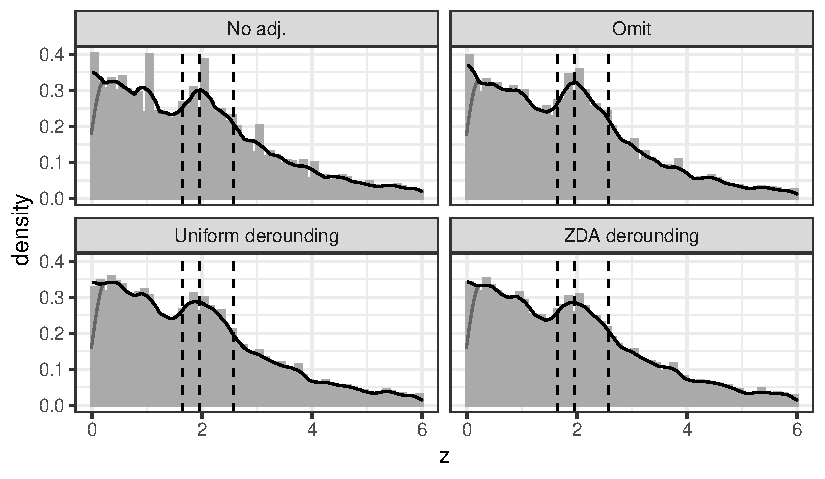
\includegraphics{C:/Users/ppuetz/Desktop/sciebo/methods_matter_replication/Submission AER/revision/comment_methods_matter/replication_repo_methods_matter_comment/Results/zplot2_all-1.pdf}

\hypertarget{did-1}{%
\subsubsection{DID}\label{did-1}}

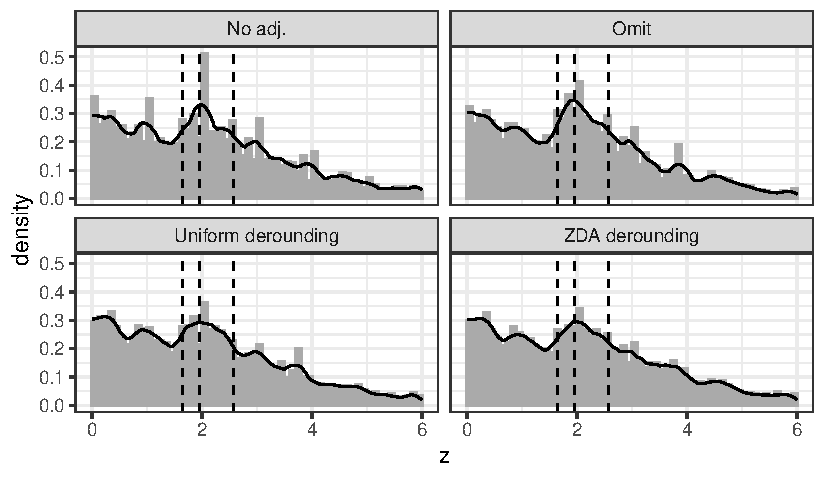
\includegraphics{C:/Users/ppuetz/Desktop/sciebo/methods_matter_replication/Submission AER/revision/comment_methods_matter/replication_repo_methods_matter_comment/Results/zplot2_did-1.pdf}

\hypertarget{iv-1}{%
\subsubsection{IV}\label{iv-1}}

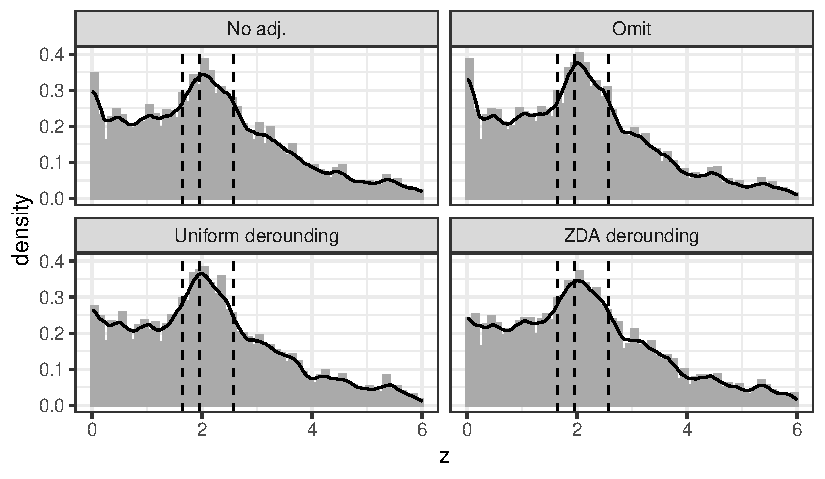
\includegraphics{C:/Users/ppuetz/Desktop/sciebo/methods_matter_replication/Submission AER/revision/comment_methods_matter/replication_repo_methods_matter_comment/Results/zplot2_iv-1.pdf}

\hypertarget{rdd-1}{%
\subsubsection{RDD}\label{rdd-1}}

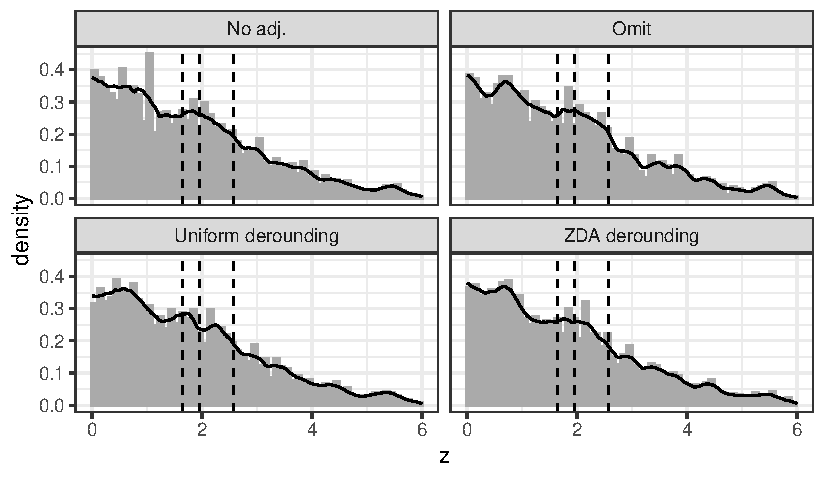
\includegraphics{C:/Users/ppuetz/Desktop/sciebo/methods_matter_replication/Submission AER/revision/comment_methods_matter/replication_repo_methods_matter_comment/Results/zplot2_rdd-1.pdf}

\hypertarget{rct-1}{%
\subsubsection{RCT}\label{rct-1}}

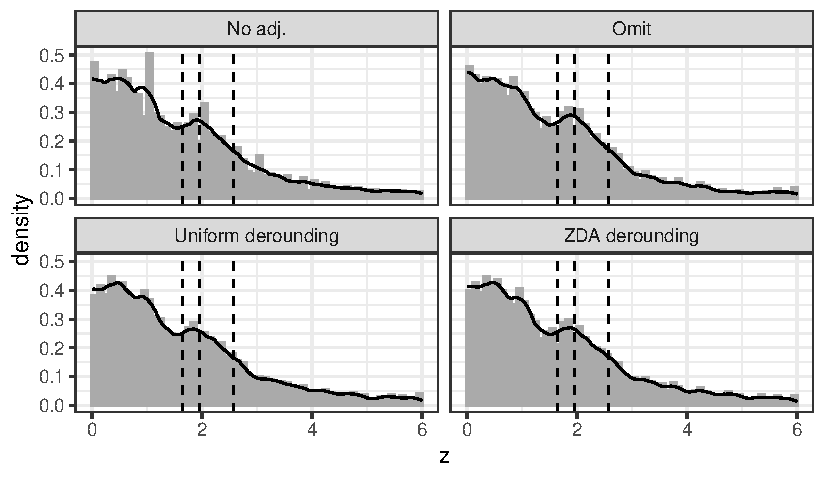
\includegraphics{C:/Users/ppuetz/Desktop/sciebo/methods_matter_replication/Submission AER/revision/comment_methods_matter/replication_repo_methods_matter_comment/Results/zplot2_rct-1.pdf}

\end{document}
